% !TeX root = main.tex

\section{Q3: Dynamics of 3R}

The dynamics (equation of motion) of a manipulator is given by the following equation

\begin{equation}
    \tau = \mathbf{M(q) \, \ddot{q} + C(q, \dot{q}) \, \dot{q} + G(q)}
    \label{eq:robot-dynamics-eq}
\end{equation}

Where

\begin{align}
    \mathbf{M} = \sum_i \left ( m_i \mathbf{J_{v_i}^\top J_{v_i} + J_{\omega_i}^\top I_{C_i} J_{\omega_i}} \right )
    &&
    \mathbf{C} = \left ( \mathbf{ \dot{M} - \frac{1}{2} \, \dot{q}^\top \frac{\partial M}{\partial q} } \right )
    &&
    \mathbf{G} = \mathbf{ \frac{\partial U}{\partial q}}
    \label{eq:robot-dynamics-eq-terms}
\end{align}

We therefore find the jacobian matrices (from forward kinematics), get the mass matrix $\mathbf{M}$, then get the coriolis and centripetal matrix $\mathbf{C}$. The gravity forces $\mathbf{G}$ is directly calculated from the potential energy. Note that the jacobian matrices $\mathbf{J_{v_i}}$ and $\mathbf{J_{\omega_i}}$ are calculated till the center of mass of the i\textsuperscript{th} link (consider a sub-manipulator).

The 3R manipulator given in the question is shown in the figure below

\begin{figure}[h]
    \centering
    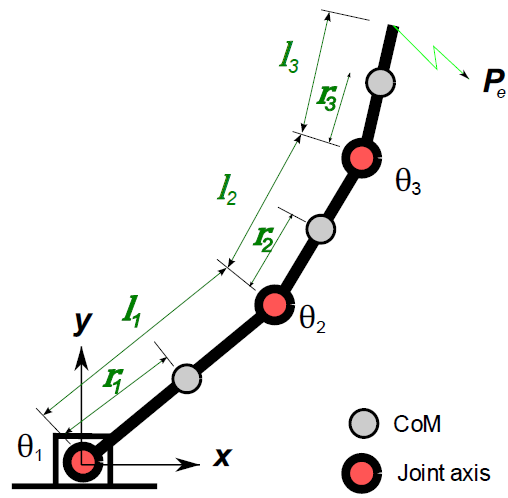
\includegraphics[width=0.3 \textwidth]{3r-dyn-img.png}
    \caption{Given 3R Manipulator}
\end{figure}

\subsection{Equation of Motion}

Refer to the program in Appendix \ref{app:3r-dyn-model-pycode} for the python code (to solve for the matrices from forward kinematics).

\subsubsection*{Forward Kinematics}

The pose of the center of mass of each link and the end effector is derived. This forward kinematics is done through visual inspection here.

\begin{align}
    \mathbf{P}_{\textup{r}_1} = \begin{bmatrix}
        r_1 c_1 \\
        r_1 s_1 \\
        \theta_1
        \end{bmatrix}
    &&
    \mathbf{P}_{\textup{r}_2} = \begin{bmatrix}
        l_1 c_1 + r_2 c_{12} \\
        l_1 s_1 + r_2 s_{12} \\
        \theta_1 + \theta_2
        \end{bmatrix}
    &&
    \mathbf{P}_{\textup{r}_3} = \begin{bmatrix}
        l_1 c_1 + l_2 c_{12} + r_3 c_{123} \\
        l_1 s_1 + l_2 s_{12} + r_3 s_{123} \\
        \theta_1 + \theta_2 + \theta_3
        \end{bmatrix}
    \label{eq:3r-fk-com}
\end{align}

The end effector is given by

\begin{align}
    \mathbf{P}_{\textup{ef}} = \begin{bmatrix}
        l_1 c_1 + l_2 c_{12} + l_3 c_{123} \\
        l_1 s_1 + l_2 s_{12} + l_3 s_{123} \\
        \theta_1 + \theta_2 + \theta_3
        \end{bmatrix}
\end{align}

Each pose is given by $\mathbf{P} = [x, y, \theta]^\top$. Each $\theta_i = q_i$.

\subsubsection*{Jacobian Matrices}

The Jacobian matrices are now calculated. Note that the linear velocity of center of mass of link $i$ is given by $\mathbf{V_{r_i}} = \mathbf{J_{v_i} \, \dot{q}}$ and the angular velocity of the center of mass of link $i$ is given by $\mathbf{\Omega_{r_i}} = \mathbf{J_{\omega_i} \, \dot{q}}$. These will be $3, 3$ matrices.

The Jacobian matrices are given by

\begin{align}
    \mathbf{J_{v_1}} &= \left[\begin{matrix}- r_{1} s_{1} & 0 & 0\\c_{1} r_{1} & 0 & 0\\0 & 0 & 0\end{matrix}\right]
    &&
    \mathbf{J_{\omega_1}} = \left[\begin{matrix}0 & 0 & 0\\0 & 0 & 0\\1 & 0 & 0\end{matrix}\right]
    \\
    \mathbf{J_{v_2}} &= \left[\begin{matrix}- l_{1} s_{1} - r_{2} s_{12} & - r_{2} s_{12} & 0\\c_{1} l_{1} + c_{12} r_{2} & c_{12} r_{2} & 0\\0 & 0 & 0\end{matrix}\right]
    &&
    \mathbf{J_{\omega_2}} = \left[\begin{matrix}0 & 0 & 0\\0 & 0 & 0\\1 & 1 & 0\end{matrix}\right]
    \\
    \mathbf{J_{v_3}} &= \left[\begin{matrix}- l_{1} s_{1} - l_{2} s_{12} - r_{3} s_{123} & - l_{2} s_{12} - r_{3} s_{123} & - r_{3} s_{123}\\c_{1} l_{1} + c_{123} r_{3} + c_{12} l_{2} & c_{123} r_{3} + c_{12} l_{2} & c_{123} r_{3}\\0 & 0 & 0\end{matrix}\right]
    &&
    \mathbf{J_{\omega_3}} = \left[\begin{matrix}0 & 0 & 0\\0 & 0 & 0\\1 & 1 & 1\end{matrix}\right]
\end{align}

\subsubsection*{Mass Matrix}

Using the above equations, we get the mass matrix as

\begin{align}
    \mathbf{M} = \sum_i \left ( m_i \mathbf{J_{v_i}^\top J_{v_i} + J_{\omega_i}^\top I_{C_i} J_{\omega_i}} \right ) = \begin{bmatrix}
        M_{11} & M_{12} & M_{13} \\
        M_{21} & M_{22} & M_{23} \\
        M_{31} & M_{32} & M_{33}
        \end{bmatrix}
    \label{eq:3r-dyn-mass-matrix}
\end{align}

Where

\begin{align}
    \begin{split}
        M_{11} =& I_{zz_1} + I_{zz_2} + I_{zz_3} + 2 c_{2} l_{1} l_{2} m_{3} + 2 c_{2} l_{1} m_{2} r_{2} + 2 c_{3} l_{2} m_{3} r_{3} + 2 c_{23} l_{1} m_{3} r_{3} + \\
            & l_{1}^{2} m_{2} + l_{1}^{2} m_{3} + l_{2}^{2} m_{3} + m_{1} r_{1}^{2} + m_{2} r_{2}^{2} + m_{3} r_{3}^{2}
    \end{split} \nonumber \\
    \begin{split}
        M_{12} =& I_{zz_2} + I_{zz_3} + c_{2} l_{1} l_{2} m_{3} + c_{2} l_{1} m_{2} r_{2} + 2 c_{3} l_{2} m_{3} r_{3} + c_{23} l_{1} m_{3} r_{3} + l_{2}^{2} m_{3} + \\
            & m_{2} r_{2}^{2} + m_{3} r_{3}^{2}
    \end{split} \nonumber \\
    \begin{split}
        M_{13} =& I_{zz_3} + c_{3} l_{2} m_{3} r_{3} + c_{23} l_{1} m_{3} r_{3} + m_{3} r_{3}^{2}
    \end{split}
    \label{eq:3r-dyn-mass-matrix-col1}
    \\
    \begin{split}
        M_{21} =& I_{zz_2} + I_{zz_3} + c_{2} l_{1} l_{2} m_{3} + c_{2} l_{1} m_{2} r_{2} + 2 c_{3} l_{2} m_{3} r_{3} + c_{23} l_{1} m_{3} r_{3} + l_{2}^{2} m_{3} + \\
            & m_{2} r_{2}^{2} + m_{3} r_{3}^{2}
    \end{split} \nonumber \\
    \begin{split}
        M_{22} =& I_{zz_2} + I_{zz_3} + 2 c_{3} l_{2} m_{3} r_{3} + l_{2}^{2} m_{3} + m_{2} r_{2}^{2} + m_{3} r_{3}^{2}
    \end{split} \nonumber \\
    \begin{split}
        M_{23} =& I_{zz_3} + c_{3} l_{2} m_{3} r_{3} + m_{3} r_{3}^{2}
    \end{split}
    \label{eq:3r-dyn-mass-matrix-col2}
    \\
    \begin{split}
        M_{31} =& I_{zz_3} + c_{3} l_{2} m_{3} r_{3} + c_{23} l_{1} m_{3} r_{3} + m_{3} r_{3}^{2}
    \end{split} \nonumber \\
    \begin{split}
        M_{32} =& I_{zz_3} + c_{3} l_{2} m_{3} r_{3} + m_{3} r_{3}^{2}
    \end{split} \nonumber \\
    \begin{split}
        M_{33} =& I_{zz_3} + m_{3} r_{3}^{2}
    \end{split}
    \label{eq:3r-dyn-mass-matrix-col3}
\end{align}

\noindent
Substitute the values in equations \ref{eq:3r-dyn-mass-matrix-col1}, \ref{eq:3r-dyn-mass-matrix-col2} and \ref{eq:3r-dyn-mass-matrix-col3} in equation \ref{eq:3r-dyn-mass-matrix} to get the \textbf{Mass Matrix} given by $\mathbf{M(q)}$

\subsubsection*{Coriolis and Centripetal Matrix}

Using \ref{eq:robot-dynamics-eq-terms}, we get the coriolis and centripetal part as

\begin{equation}
    \mathbf{C(q, \dot{q}) \, \dot{q}} = \left ( \mathbf{ \dot{M} - \frac{1}{2} \, \dot{q}^\top \frac{\partial M}{\partial q} } \right ) \, \mathbf{\dot{q}} = \mathbf{\dot{M} \, \dot{q}} - \frac{1}{2} \begin{bmatrix}
        \mathbf{\dot{q}^\top} \frac{\partial \mathbf{M}}{\partial q_1} \mathbf{\dot{q}} \\
        \vdots \\
        \mathbf{\dot{q}^\top} \frac{\partial \mathbf{M}}{\partial q_n} \mathbf{\dot{q}}
        \end{bmatrix} 
    = \mathbf{\dot{M} \, \dot{q}} - \frac{1}{2} \begin{bmatrix}
        \mathbf{\dot{q}^\top} \frac{\partial \mathbf{M}}{\partial q_1} \mathbf{\dot{q}} \\
        \mathbf{\dot{q}^\top} \frac{\partial \mathbf{M}}{\partial q_2} \mathbf{\dot{q}} \\
        \mathbf{\dot{q}^\top} \frac{\partial \mathbf{M}}{\partial q_3} \mathbf{\dot{q}}
        \end{bmatrix}
\end{equation}

Calculating the time derivative of the mass matrix is done as follows

\begin{equation}
    \frac{\mathrm{d} \mathbf{M}}{\mathrm{d} t} = \mathbf{\dot{M}} = \begin{bmatrix}
        \frac{\mathrm{d} M_{11}}{\mathrm{d} t} & \frac{\mathrm{d} M_{12}}{\mathrm{d} t} & \frac{\mathrm{d} M_{13}}{\mathrm{d} t} \\
        \frac{\mathrm{d} M_{21}}{\mathrm{d} t} & \frac{\mathrm{d} M_{22}}{\mathrm{d} t} & \frac{\mathrm{d} M_{23}}{\mathrm{d} t} \\
        \frac{\mathrm{d} M_{31}}{\mathrm{d} t} & \frac{\mathrm{d} M_{32}}{\mathrm{d} t} & \frac{\mathrm{d} M_{33}}{\mathrm{d} t}
        \end{bmatrix}
\end{equation}

The derivative of element $i, j$ can be simplified as follows

\begin{equation}
    \frac{\mathrm{d} M_{ij}}{\mathrm{d} t} = \frac{\mathrm{d} M_{ij}}{\mathrm{d} q_1} \frac{\mathrm{d} q_1}{\mathrm{d} t} + \frac{\mathrm{d} M_{ij}}{\mathrm{d} q_2} \frac{\mathrm{d} q_2}{\mathrm{d} t} + \frac{\mathrm{d} M_{ij}}{\mathrm{d} q_3} \frac{\mathrm{d} q_3}{\mathrm{d} t} = M_{ij1} \frac{\mathrm{d} q_1}{\mathrm{d} t} + M_{ij2} \frac{\mathrm{d} q_2}{\mathrm{d} t} + M_{ij3} \frac{\mathrm{d} q_3}{\mathrm{d} t}
\end{equation}

The coriolis and centripetal matrix is therefore achieved as

\begin{align}
    \mathbf{C} = \left ( \mathbf{ \dot{M} - \frac{1}{2} \, \dot{q}^\top \frac{\partial M}{\partial q} } \right ) = \begin{bmatrix}
        C_{11} & C_{12} & C_{13} \\
        C_{21} & C_{22} & C_{23} \\
        C_{31} & C_{32} & C_{33}
        \end{bmatrix}
    \label{eq:3r-dyn-cc-matrix}
\end{align}

Where

\begin{align}
    \begin{split}
        C_{11} =& - 2 \dot{q}_2 l_{1} l_{2} m_{3} s_{2} - 2 \dot{q}_2 l_{1} m_{2} r_{2} s_{2} - 2 \dot{q}_3 l_{2} m_{3} r_{3} s_{3} - 2 l_{1} m_{3} r_{3} s_{23} \left(\dot{q}_2 + \dot{q}_3\right)
    \end{split} \nonumber \\
    \begin{split}
        C_{12} =& - \dot{q}_2 l_{1} l_{2} m_{3} s_{2} - \dot{q}_2 l_{1} m_{2} r_{2} s_{2} - 2 \dot{q}_3 l_{2} m_{3} r_{3} s_{3} - l_{1} m_{3} r_{3} s_{23} \left(\dot{q}_2 + \dot{q}_3\right)
    \end{split} \nonumber \\
    \begin{split}
        C_{13} =& - m_{3} r_{3} \left(\dot{q}_3 l_{2} s_{3} + l_{1} s_{23} \left(\dot{q}_2 + \dot{q}_3\right)\right)
    \end{split}
    \label{eq:3r-dyn-cc-matrix-col1}
    \\
    \begin{split}
        C_{21} =& 1.0 \dot{q}_1 l_{1} l_{2} m_{3} s_{2} + 1.0 \dot{q}_1 l_{1} m_{2} r_{2} s_{2} + 1.0 \dot{q}_1 l_{1} m_{3} r_{3} s_{23} - 0.5 \dot{q}_2 l_{1} l_{2} m_{3} s_{2} - 0.5 \dot{q}_2 l_{1} m_{2} r_{2} s_{2} - \\
            & 0.5 \dot{q}_2 l_{1} m_{3} r_{3} s_{23} - 0.5 \dot{q}_3 l_{1} m_{3} r_{3} s_{23} - 2.0 \dot{q}_3 l_{2} m_{3} r_{3} s_{3}
    \end{split} \nonumber \\
    \begin{split}
        C_{22} =& 0.5 \dot{q}_1 l_{1} \left(l_{2} m_{3} s_{2} + m_{2} r_{2} s_{2} + m_{3} r_{3} s_{23}\right) - 2 \dot{q}_3 l_{2} m_{3} r_{3} s_{3}
    \end{split} \nonumber \\
    \begin{split}
        C_{23} =& m_{3} r_{3} \left(0.5 \dot{q}_1 l_{1} s_{23} - \dot{q}_3 l_{2} s_{3}\right)
    \end{split}
    \label{eq:3r-dyn-cc-matrix-col2}
    \\
    \begin{split}
        C_{31} =& m_{3} r_{3} \left(1.0 \dot{q}_1 l_{1} s_{23} + 1.0 \dot{q}_1 l_{2} s_{3} - 0.5 \dot{q}_2 l_{1} s_{23} + 1.0 \dot{q}_2 l_{2} s_{3} - 0.5 \dot{q}_3 l_{1} s_{23} - 0.5 \dot{q}_3 l_{2} s_{3}\right)
    \end{split} \nonumber \\
    \begin{split}
        C_{32} =& m_{3} r_{3} \left(0.5 \dot{q}_1 \left(l_{1} s_{23} + 2 l_{2} s_{3}\right) + 1.0 \dot{q}_2 l_{2} s_{3} - 0.5 \dot{q}_3 l_{2} s_{3}\right)
    \end{split} \nonumber \\
    \begin{split}
        C_{33} =& 0.5 m_{3} r_{3} \left(\dot{q}_1 \left(l_{1} s_{23} + l_{2} s_{3}\right) + \dot{q}_2 l_{2} s_{3}\right)
    \end{split}
    \label{eq:3r-dyn-cc-matrix-col3}
\end{align}

\noindent
Substitute the values in equations \ref{eq:3r-dyn-cc-matrix-col1}, \ref{eq:3r-dyn-cc-matrix-col2} and \ref{eq:3r-dyn-cc-matrix-col3} in equation \ref{eq:3r-dyn-cc-matrix} to get the \textbf{Coriolis and Centripetal Matrix} given by $\mathbf{C(q, \dot{q})}$.

\subsubsection*{Gravity Vector}

We first calculate the potential energy of the system: we use the $y$ value of the poses $\mathbf{P}_{\textup{r}_i}$ (), then using \ref{eq:robot-dynamics-eq-terms}, we get the gravity vector $\mathbf{G(q)}$. The potential energy is given by

\begin{align}
    \mathbf{U} &= - \left ( m_1 \, g \, \mathbf{P}_{\textup{r}_1}[y] + m_2 \, g \, \mathbf{P}_{\textup{r}_2}[y] + m_3 \, g \, \mathbf{P}_{\textup{r}_3}[y] \right )
    \nonumber \\
    &= - g \left(l_{1} m_{2} s_{1} + l_{1} m_{3} s_{1} + l_{2} m_{3} s_{12} + m_{1} r_{1} s_{1} + m_{2} r_{2} s_{12} + m_{3} r_{3} s_{123}\right)
\end{align}

The partial derivative with respect to $\mathbf{q}$ yields the gravity vector, which is given by

\begin{equation}
    \mathbf{G(q)} = \mathbf{ \frac{\partial U}{\partial q}} = \begin{bmatrix}
        G_1 \\ G_2 \\ G_3
        \end{bmatrix} = \begin{bmatrix}
        - g \left(c_{1} l_{1} m_{2} + c_{1} l_{1} m_{3} + c_{1} m_{1} r_{1} + c_{123} m_{3} r_{3} + c_{12} l_{2} m_{3} + c_{12} m_{2} r_{2}\right) \\
        - g \left(c_{123} m_{3} r_{3} + c_{12} l_{2} m_{3} + c_{12} m_{2} r_{2}\right) \\
        - c_{123} g m_{3} r_{3}
        \end{bmatrix}
        \label{eq:3r-dyn-gravity-vect}
\end{equation}

\noindent
The equation \ref{eq:3r-dyn-gravity-vect} gives the \textbf{Gravity Vector} given by $\mathbf{G(q)}$.

\subsubsection*{Equation of Motion}

The joint efforts (torques) $\tau$ are given by

\begin{align}
    \tau =& \mathbf{M(q) \, \ddot{q} + C(q, \dot{q}) \, \dot{q} + G(q)} \\
    =& \begin{bmatrix}
        M_{11} & M_{12} & M_{13} \\
        M_{21} & M_{22} & M_{23} \\
        M_{31} & M_{32} & M_{33}
        \end{bmatrix} \begin{bmatrix}
            \ddot{q}_1 \\ \ddot{q}_2 \\ \ddot{q}_3
            \end{bmatrix}
    + \begin{bmatrix}
        C_{11} & C_{12} & C_{13} \\
        C_{21} & C_{22} & C_{23} \\
        C_{31} & C_{32} & C_{33}
        \end{bmatrix} \begin{bmatrix}
            \dot{q}_1 \\ \dot{q}_2 \\ \dot{q}_3
            \end{bmatrix}
    + \begin{bmatrix}
        G_1 \\ G_2 \\ G_3
        \end{bmatrix}
    = \begin{bmatrix}
        \tau_1 \\ \tau_2 \\ \tau_3
        \end{bmatrix}
    \label{eq:3r-dyn-tau-vect}
\end{align}

Where

\begin{align}
    \begin{split}
        \tau_1 =& \ddot{q}_1 \left(I_{zz_1} + I_{zz_2} + I_{zz_3} + 2 c_{2} l_{1} l_{2} m_{3} + 2 c_{2} l_{1} m_{2} r_{2} + 2 c_{3} l_{2} m_{3} r_{3} + 2 c_{23} l_{1} m_{3} r_{3} + l_{1}^{2} m_{2} + l_{1}^{2} m_{3} \right.\\
            & \left. + l_{2}^{2} m_{3} + m_{1} r_{1}^{2} + m_{2} r_{2}^{2} + m_{3} r_{3}^{2}\right) + \ddot{q}_2 \left(I_{zz_2} + I_{zz_3} + c_{2} l_{1} l_{2} m_{3} + c_{2} l_{1} m_{2} r_{2} + 2 c_{3} l_{2} m_{3} r_{3} \right. \\
            & \left. + c_{23} l_{1} m_{3} r_{3} + l_{2}^{2} m_{3} + m_{2} r_{2}^{2} + m_{3} r_{3}^{2}\right) + \ddot{q}_3 \left(I_{zz_3} + c_{3} l_{2} m_{3} r_{3} + c_{23} l_{1} m_{3} r_{3} + m_{3} r_{3}^{2}\right) \\
            & - 2 \dot{q}_1 \left(\dot{q}_2 l_{1} l_{2} m_{3} s_{2} + \dot{q}_2 l_{1} m_{2} r_{2} s_{2} + \dot{q}_3 l_{2} m_{3} r_{3} s_{3} + l_{1} m_{3} r_{3} s_{23} \left(\dot{q}_2 + \dot{q}_3\right)\right) - \dot{q}_2 \left(\dot{q}_2 l_{1} l_{2} m_{3} s_{2} \right. \\
            & \left. + \dot{q}_2 l_{1} m_{2} r_{2} s_{2} + 2 \dot{q}_3 l_{2} m_{3} r_{3} s_{3} + l_{1} m_{3} r_{3} s_{23} \left(\dot{q}_2 + \dot{q}_3\right)\right) - \dot{q}_3 m_{3} r_{3} \left(\dot{q}_3 l_{2} s_{3} + l_{1} s_{23} \left(\dot{q}_2 + \dot{q}_3\right)\right) \\
            & - g \left(c_{1} l_{1} m_{2} + c_{1} l_{1} m_{3} + c_{1} m_{1} r_{1} + c_{123} m_{3} r_{3} + c_{12} l_{2} m_{3} + c_{12} m_{2} r_{2}\right)
    \end{split}
    \label{eq:3r-dyn-tau-vect-elem1}
    \\
    \begin{split}
        \tau_2 =& 1.0 I_{zz_2} \ddot{q}_1 + 1.0 I_{zz_2} \ddot{q}_2 + 1.0 I_{zz_3} \ddot{q}_1 + 1.0 I_{zz_3} \ddot{q}_2 + 1.0 I_{zz_3} \ddot{q}_3 + 1.0 \ddot{q}_1 c_{2} l_{1} l_{2} m_{3} + 1.0 \ddot{q}_1 c_{2} l_{1} m_{2} r_{2} \\
            & + 2.0 \ddot{q}_1 c_{3} l_{2} m_{3} r_{3} + 1.0 \ddot{q}_1 c_{23} l_{1} m_{3} r_{3} + 1.0 \ddot{q}_1 l_{2}^{2} m_{3} + 1.0 \ddot{q}_1 m_{2} r_{2}^{2} + 1.0 \ddot{q}_1 m_{3} r_{3}^{2} + 2.0 \ddot{q}_2 c_{3} l_{2} m_{3} r_{3} \\
            & + 1.0 \ddot{q}_2 l_{2}^{2} m_{3} + 1.0 \ddot{q}_2 m_{2} r_{2}^{2} + 1.0 \ddot{q}_2 m_{3} r_{3}^{2} + 1.0 \ddot{q}_3 c_{3} l_{2} m_{3} r_{3} + 1.0 \ddot{q}_3 m_{3} r_{3}^{2} + 1.0 \dot{q}_1^{2} l_{1} l_{2} m_{3} s_{2} \\
            & + 1.0 \dot{q}_1^{2} l_{1} m_{2} r_{2} s_{2} + 1.0 \dot{q}_1^{2} l_{1} m_{3} r_{3} s_{23} - 2.0 \dot{q}_1 \dot{q}_3 l_{2} m_{3} r_{3} s_{3} - 2.0 \dot{q}_2 \dot{q}_3 l_{2} m_{3} r_{3} s_{3} - 1.0 \dot{q}_3^{2} l_{2} m_{3} r_{3} s_{3} \\
            & - 1.0 c_{123} g m_{3} r_{3} - 1.0 c_{12} g l_{2} m_{3} - 1.0 c_{12} g m_{2} r_{2}
    \end{split}
    \label{eq:3r-dyn-tau-vect-elem2}
    \\
    \begin{split}
        \tau_3 =& 1.0 I_{zz_3} \ddot{q}_1 + 1.0 I_{zz_3} \ddot{q}_2 + 1.0 I_{zz_3} \ddot{q}_3 + 1.0 \ddot{q}_1 c_{3} l_{2} m_{3} r_{3} + 1.0 \ddot{q}_1 c_{23} l_{1} m_{3} r_{3} + 1.0 \ddot{q}_1 m_{3} r_{3}^{2} \\
            & + 1.0 \ddot{q}_2 c_{3} l_{2} m_{3} r_{3} + 1.0 \ddot{q}_2 m_{3} r_{3}^{2} + 1.0 \ddot{q}_3 m_{3} r_{3}^{2} + 1.0 \dot{q}_1^{2} l_{1} m_{3} r_{3} s_{23} + 1.0 \dot{q}_1^{2} l_{2} m_{3} r_{3} s_{3} \\
            & + 2.0 \dot{q}_1 \dot{q}_2 l_{2} m_{3} r_{3} s_{3} + 1.0 \dot{q}_2^{2} l_{2} m_{3} r_{3} s_{3} - 1.0 c_{123} g m_{3} r_{3}
    \end{split}
    \label{eq:3r-dyn-tau-vect-elem3}
\end{align}

Substituting the values in equations \ref{eq:3r-dyn-tau-vect-elem1}, \ref{eq:3r-dyn-tau-vect-elem2} and \ref{eq:3r-dyn-tau-vect-elem3} in equation \ref{eq:3r-dyn-tau-vect}, we get the joint efforts (equations of motion) $\tau$.

\subsection{Symmetric Mass Matrix}

From equation \ref{eq:3r-dyn-mass-matrix}, it is evident that $M_{12} = M_{21}$, $M_{13} = M_{31}$ and $M_{23} = M_{32}$. Therefore $\mathbf{M} = \mathbf{M}^\top$, in other words, the mass matrix is a \textbf{symmetric matrix}.

Since $\mathbf{M} = \mathbf{M}^\top$,

\begin{equation}
    \mathbf{M} = \mathbf{M}^\top
    \Rightarrow \mathbf{M} - \mathbf{M}^\top = \mathbf{0}
\end{equation}

This is also verified through the program in appendix \ref{app:3r-dyn-model-pycode}.

\subsection{Skew-Symmetric matrix in model}

A matrix $A$ is skew symmetric if $A = -A^\top$. 

Deriving the Equation of motion for an open-chain manipulator

\begin{align}
    L(\theta, \dot{\theta}) = \frac{1}{2} \dot{\theta}^\top M(\theta) \dot{\theta} - V(\theta)
    &&
    \frac{d}{dt} \frac{\partial L}{\partial \dot{\theta}_i} - \frac{\partial L}{\partial \theta_i} = \Upsilon_i
    \nonumber \\
    \frac{d}{dt} \frac{\partial L}{\partial \dot{\theta}_i} = \frac{d}{dt} \left ( \sum_{j=1}^{n} M_{ij} \dot{\theta}_j  \right ) = \sum_{j=1}^{n} \left ( M_{ij} \ddot{\theta}_j + \dot{M}_{ij} \dot{\theta}_j \right )
    \nonumber \\
    \frac{\partial L}{\partial \theta_i} = \frac{1}{2} \sum_{j,k=1}^{n} \frac{\partial M_{kj}}{\partial \theta_i} \dot{\theta}_k \dot{\theta}_j - \frac{\partial V}{\partial \theta_i}
    \nonumber \\
    \sum_{j=1}^{n} M_{ij} \ddot{\theta}_j + \sum_{j,k=1}^{n} \left ( \frac{\partial M_{ij}}{\partial \theta_k} \dot{\theta}_j \dot{\theta}_k - \frac{1}{2} \frac{\partial M_{kj}}{\partial \theta_i} \dot{\theta}_k \dot{\theta}_j \right ) + \frac{\partial V}{\partial \theta_i} (\theta) = \Upsilon_i
\end{align}

From the model of the Coriolis matrix, it can be written in terms of Christoffel symbols as follows

\begin{equation}
    C(q, \dot{q}) := \left \{ c_{ij} \right \} = \frac{1}{2} \left \{ \sum_{k=1}^{n} \left ( \frac{\partial m_{ij}}{\partial q_k} + \frac{\partial m_{ki}}{\partial q_j} - \frac{\partial m_{kj}}{\partial q_i}\right ) \dot{q}_k \right \}
\end{equation}

Where $M(q) = \left \{ m_{ij} \right \}$ is the mass matrix. Using this, it can be shown that $(\dot{M} - 2C)$ is skew symmetric.

\begin{align}
    \left ( \dot{M} - 2C \right )_{ij} =& \dot{M}_{ij} (\theta) - 2 C_{ij} (\theta) \\
    =& \sum_{k=1}^{n} \frac{\partial M_{ij}}{\partial \theta_k} \dot{\theta}_k - \frac{\partial M_{ij}}{\partial \theta_k} \dot{\theta}_k - \frac{\partial M_{ik}}{\partial \theta_j} \dot{\theta}_k + \frac{\partial M_{kj}}{\partial \theta_i} \dot{\theta}_k \\
    =& \sum_{k=1}^{n} \frac{\partial M_{kj}}{\partial \theta_i} \dot{\theta}_k - \frac{\partial M_{ik}}{\partial \theta_j} \dot{\theta}_k
\end{align}

Switching $i$ and $j$ shows that $\left ( \dot{M} - 2C \right )^\top = -\left ( \dot{M} - 2C \right )$. This proof is from the section 3.2 of Murray-1994 \footnote{Murray, R.M., Li, Z., and Sastry, S. (1994). \textit{A Mathematical
Introduction to Robotic Manipulation}. CRC Press}.

However, for the matrices defined above, the matrix $\left ( \dot{M} - 2C \right )$ does not appear to come out as a skew symmetric matrix. This may be because of the choice of $C$. Check the output at the end of appendix \ref{app:3r-dyn-model-pycode} and the resultant matrix in equation \ref{eq:app-3r-dyn-ssm-mat}. To obtain a skew symmetric matrix, we use the Cristoffel symbols.

\subsubsection*{Cristoffel Symbols}

We use the following equation for the new Coriolis matrix (a better method to find the coriolis matrix)

\begin{equation}
    \mathbf{C}_{\textup{cris}} := \left \{ c_{ij} \right \} = \left \{ \frac{1}{2} \sum_{k=1}^{n} \left ( \frac{\partial m_{ij}}{\partial q_k} + \frac{\partial m_{ki}}{\partial q_j} - \frac{\partial m_{kj}}{\partial q_i}\right ) \dot{q}_k \right \}
\end{equation}


Following the above (see the last segment of code in Appendix \ref{app:3r-dyn-model-pycode}), we get

\begin{align}
    \mathbf{C}_{\textup{cris}} = \begin{bmatrix}
        V_{11} & V_{12} & V_{13} \\
        V_{21} & V_{22} & V_{23} \\
        V_{31} & V_{32} & V_{33}
        \end{bmatrix}
    \label{eq:3r-dyn-cc-cris-matrix}
\end{align}

Where

\begin{align}
    \begin{split}
        V_{11} =& - 1.0 \dot{q}_2 l_{1} \left(l_{2} m_{3} s_{2} + m_{2} r_{2} s_{2} + m_{3} r_{3} s_{23}\right) - 1.0 \dot{q}_3 m_{3} r_{3} \left(l_{1} s_{23} + l_{2} s_{3}\right)
    \end{split}
    \nonumber \\
    \begin{split}
        V_{12} =& - 1.0 \dot{q}_1 l_{1} \left(l_{2} m_{3} s_{2} + m_{2} r_{2} s_{2} + m_{3} r_{3} s_{23}\right) - 1.0 \dot{q}_2 l_{1} \left(l_{2} m_{3} s_{2} + m_{2} r_{2} s_{2} + m_{3} r_{3} s_{23}\right) -\\
            & 1.0 \dot{q}_3 m_{3} r_{3} \left(l_{1} s_{23} + l_{2} s_{3}\right)
    \end{split}
    \nonumber \\
    \begin{split}
        V_{13} =& - 1.0 m_{3} r_{3} \left(l_{1} s_{23} + l_{2} s_{3}\right) \left(\dot{q}_1 + \dot{q}_2 + \dot{q}_3\right)
    \end{split}
    \label{eq:3r-dyn-cc-cris-matrix-row1} \\
    \begin{split}
        V_{21} =& \dot{q}_1 l_{1} \left(l_{2} m_{3} s_{2} + m_{2} r_{2} s_{2} + m_{3} r_{3} s_{23}\right) - 1.0 \dot{q}_3 l_{2} m_{3} r_{3} s_{3}
    \end{split}
    \nonumber \\
    \begin{split}
        V_{22} =& - 1.0 \dot{q}_3 l_{2} m_{3} r_{3} s_{3}
    \end{split}
    \nonumber \\
    \begin{split}
        V_{23} =& - 1.0 l_{2} m_{3} r_{3} s_{3} \left(\dot{q}_1 + \dot{q}_2 + \dot{q}_3\right)
    \end{split}
    \label{eq:3r-dyn-cc-cris-matrix-row2} \\
    \begin{split}
        V_{31} =& m_{3} r_{3} \left(\dot{q}_1 \left(l_{1} s_{23} + l_{2} s_{3}\right) + 1.0 \dot{q}_2 l_{2} s_{3}\right)
    \end{split}
    \nonumber \\
    \begin{split}
        V_{32} =& 1.0 l_{2} m_{3} r_{3} s_{3} \left(\dot{q}_1 + \dot{q}_2\right)
    \end{split}
    \nonumber \\
    \begin{split}
        V_{33} =& 0
    \end{split}
    \label{eq:3r-dyn-cc-cris-matrix-row3}
\end{align}

Substitute the equations \ref{eq:3r-dyn-cc-cris-matrix-row1}, \ref{eq:3r-dyn-cc-cris-matrix-row2}, \ref{eq:3r-dyn-cc-cris-matrix-row3} in equation \ref{eq:3r-dyn-cc-cris-matrix} to get the new coriolis matrix $\mathbf{C}_{\textup{cris}}$ through Cristoffel symbols.

In Appendix \ref{app:3r-dyn-model-pycode}, through $\textup{ssm}_{\textup{cris}}$, it is verified that $\mathbf{\dot{M}} - 2\mathbf{C}_{\textup{cris}}$ is a skew symmetric matrix. Check equation \ref{eq:app-3r-dyn-ssm-cris-mat} for the proof of this.
